\documentclass{beamer}

%% --------------------------------------------------
%% preamble

\usepackage{graphicx}
% \usepackage{tabularx}
\usetheme{Warsaw}
\usecolortheme{whale}
\AtBeginSection[]
{
  \begin{frame}
    \frametitle{Table of Contents}
    \tableofcontents[currentsection]
  \end{frame}
}
\AtBeginSubsection[]
{
  \begin{frame}
    \frametitle{Table of Contents}
    \tableofcontents[currentsection,currentsubsection]
  \end{frame}
}

%% --------------------------------------------------
%% title page info

\title{How to Technologically tame the financial markets!}
\author{Pradnyesh Sawant}
\date{May 25-26, 2017}

%% --------------------------------------------------
%% document begins here

\begin{document}

%% -------------------------
%% title page is actually shown here
\frame{\titlepage}

\begin{frame}
  \frametitle{The real title}
  Things I wish someone would have told me at the begining of my career ;)
\end{frame}

%% -------------------------
%% About Me
\section{About Me}
\begin{frame}
  \frametitle{My Family}
  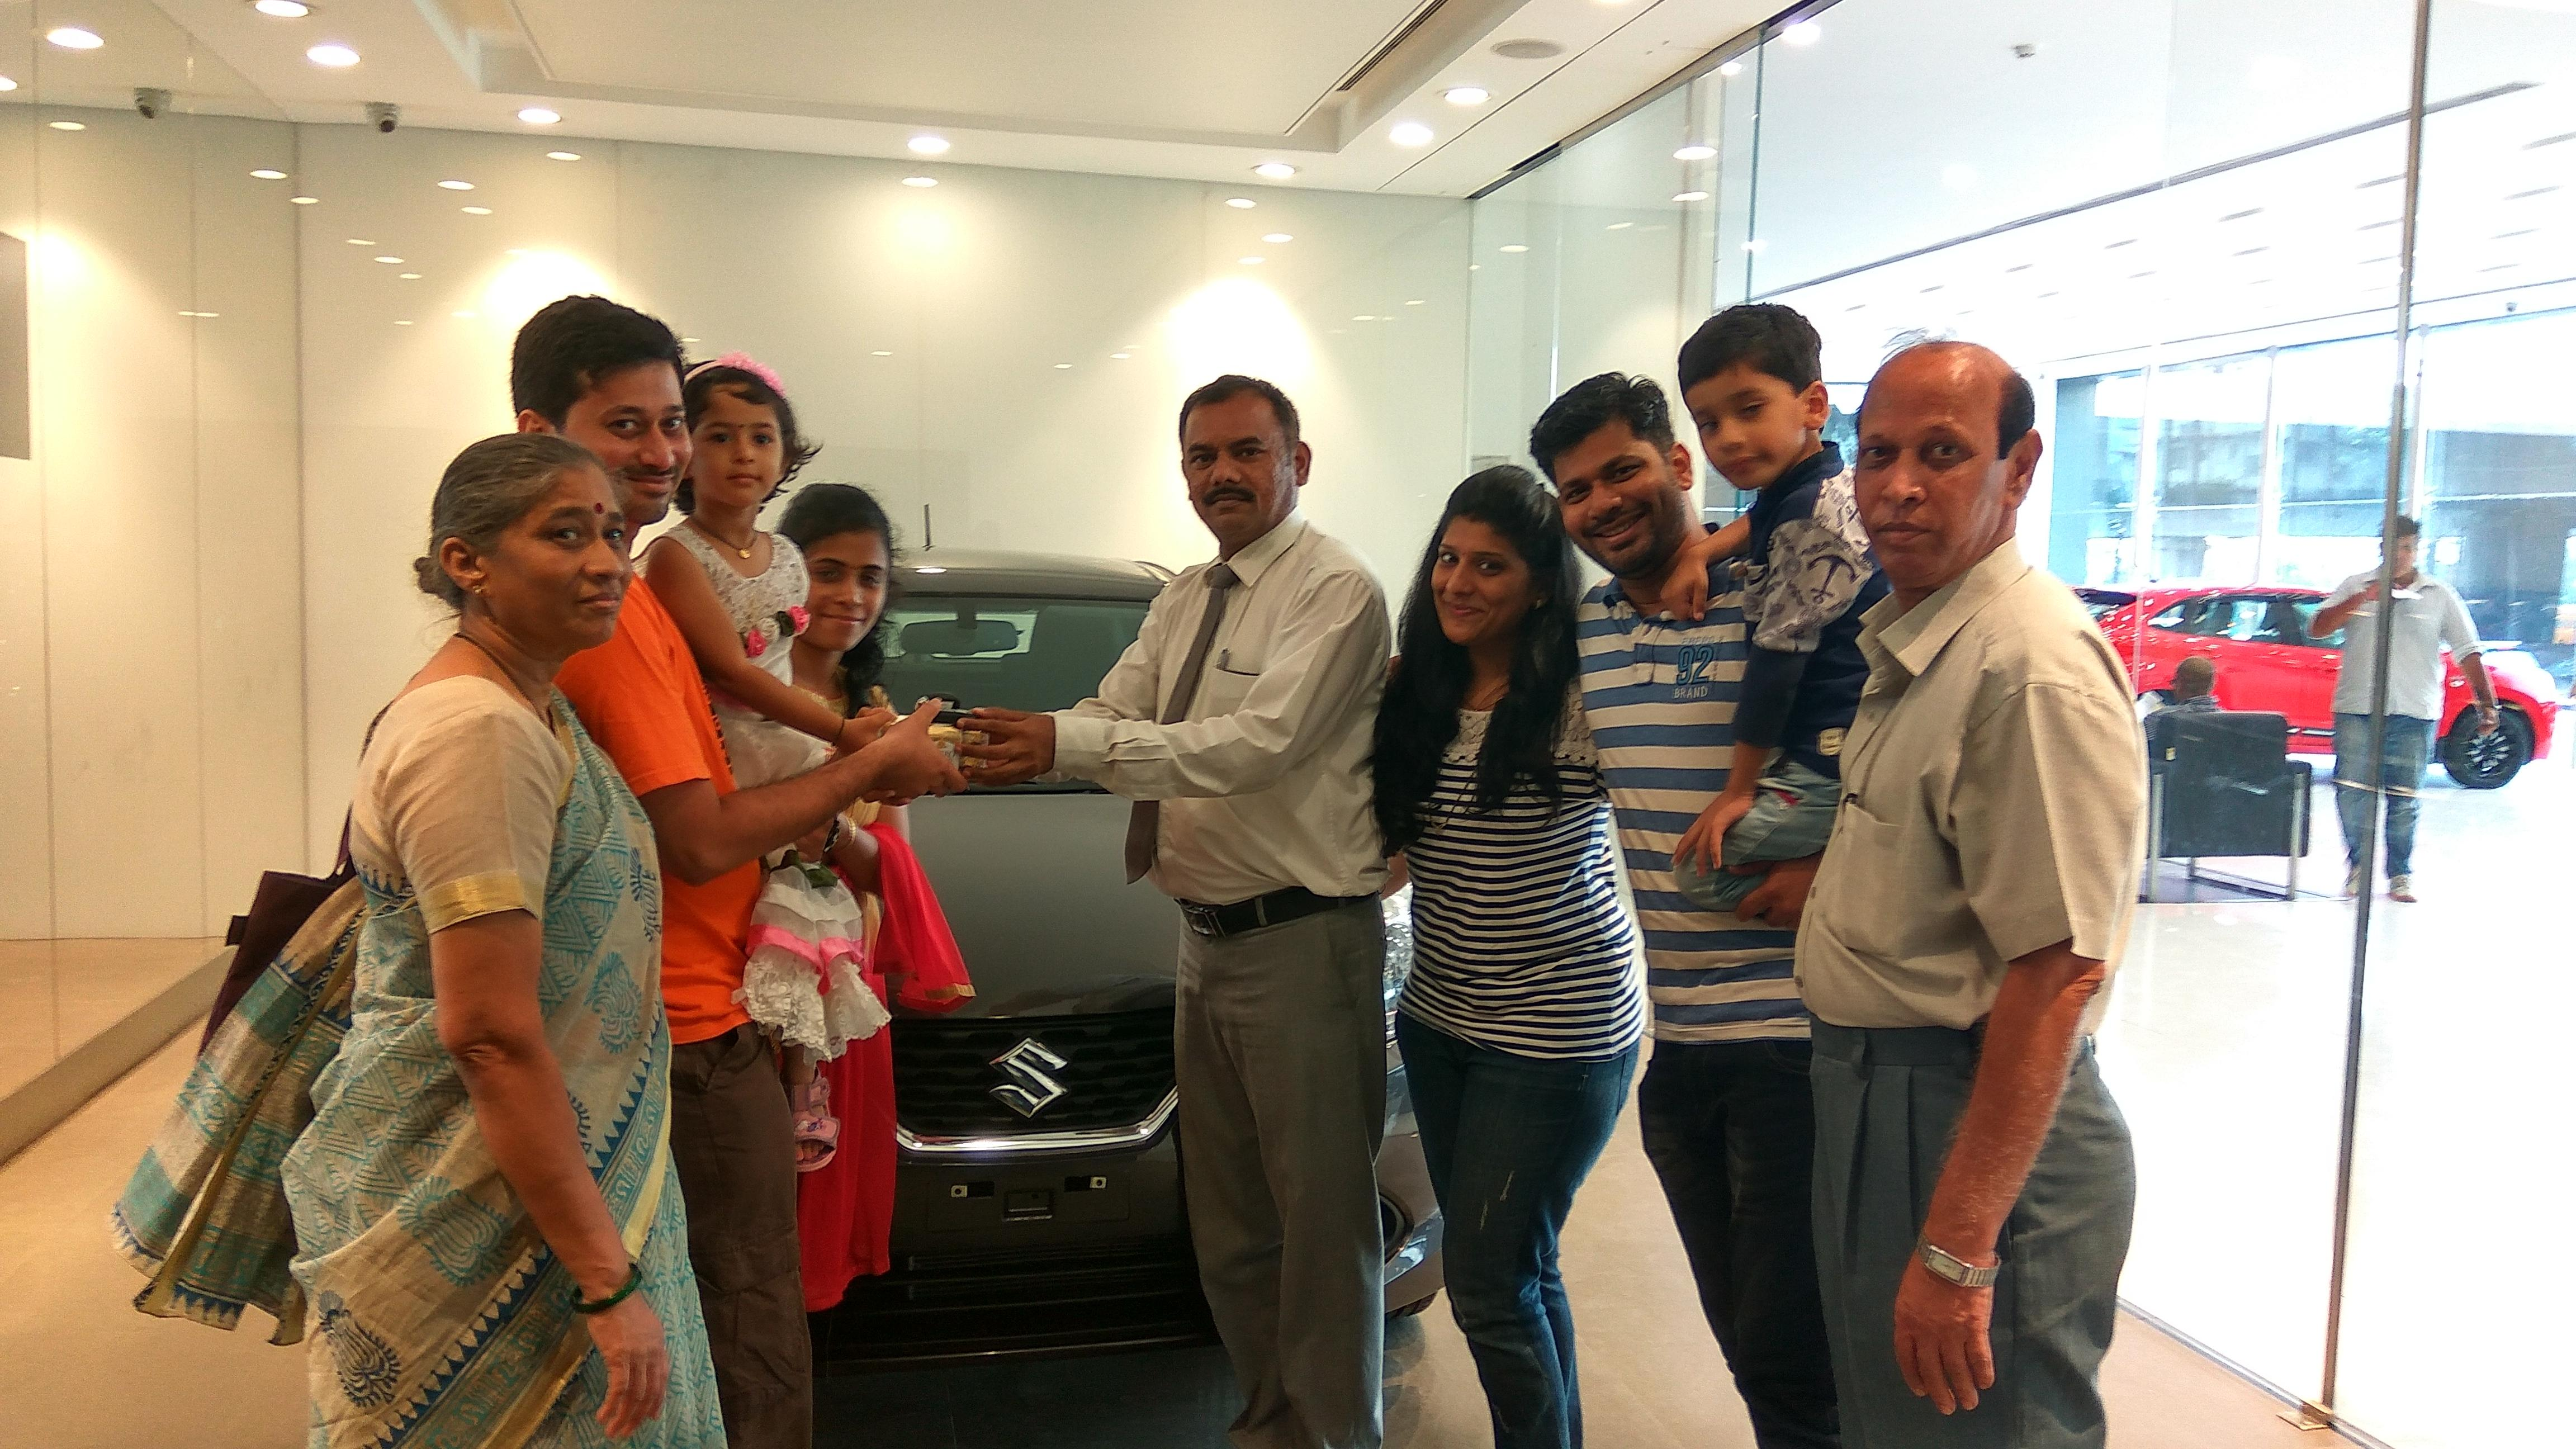
\includegraphics[height=5.4cm,width=10.8cm]{IMG_20160618_175653_HDR.jpg}
\end{frame}
\begin{frame}
  \frametitle{Education and Career}
  \begin{tabular}{ l  l  l  l }
    \textbf{From} & \textbf{To} & \textbf{What} & \textbf{Where}\\
    & & & \\
    1999 & 2003 & Student & B.E. @ Mumbai University\\
    2003 & 2005 & Assoc. Software Analyst & Nse.iT\\
    2005 & 2007 & Student & MTech @ IITG\\
    2007 & 2012 & Principal Engineer & Yahoo! SDC\\
    2012 & 2014 & Engineering Manager & Samsung Electronics (HQ)\\
    2014 & 2016 & Founder & Gryff!n SD LLP\\
    2016 & Present & Head of Engineering & Mindseed Preschool\\
  \end{tabular}
\end{frame}
\begin{frame}
  \frametitle{Growth}
  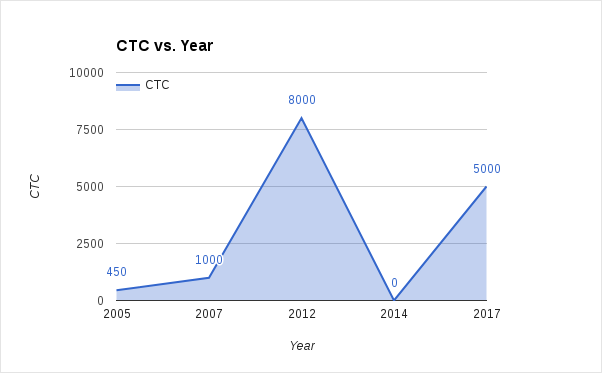
\includegraphics[height=5.4cm,width=10.8cm]{screenshot_2017-05-19_08-08-01.png}

  more than 10x growth between 2005 and 2017 (12 years)
\end{frame}
\begin{frame}
  \frametitle{Lessons Learned}
  \begin{itemize}[<+->]
  \item Investment in career will outperform any other investment! -- anonymous
  \item The only people really interested in your career are yourself and your mother. -- Carol Bartz (Former CEO of Yahoo!)
  \end{itemize}
\end{frame}

%% -------------------------
%% Financial markets
\section{Financial markets}
%% ----------
\subsection{Introduction}
\begin{frame}
  \frametitle{Introduction}
  \begin{itemize}[<+->]
  \item Stock Market
  \item Prediction of time-series data using Machine Learning techniques
  \end{itemize}
\end{frame}
%% ----------
\subsection{Product : what}
\begin{frame}
  \frametitle{Home Page}
  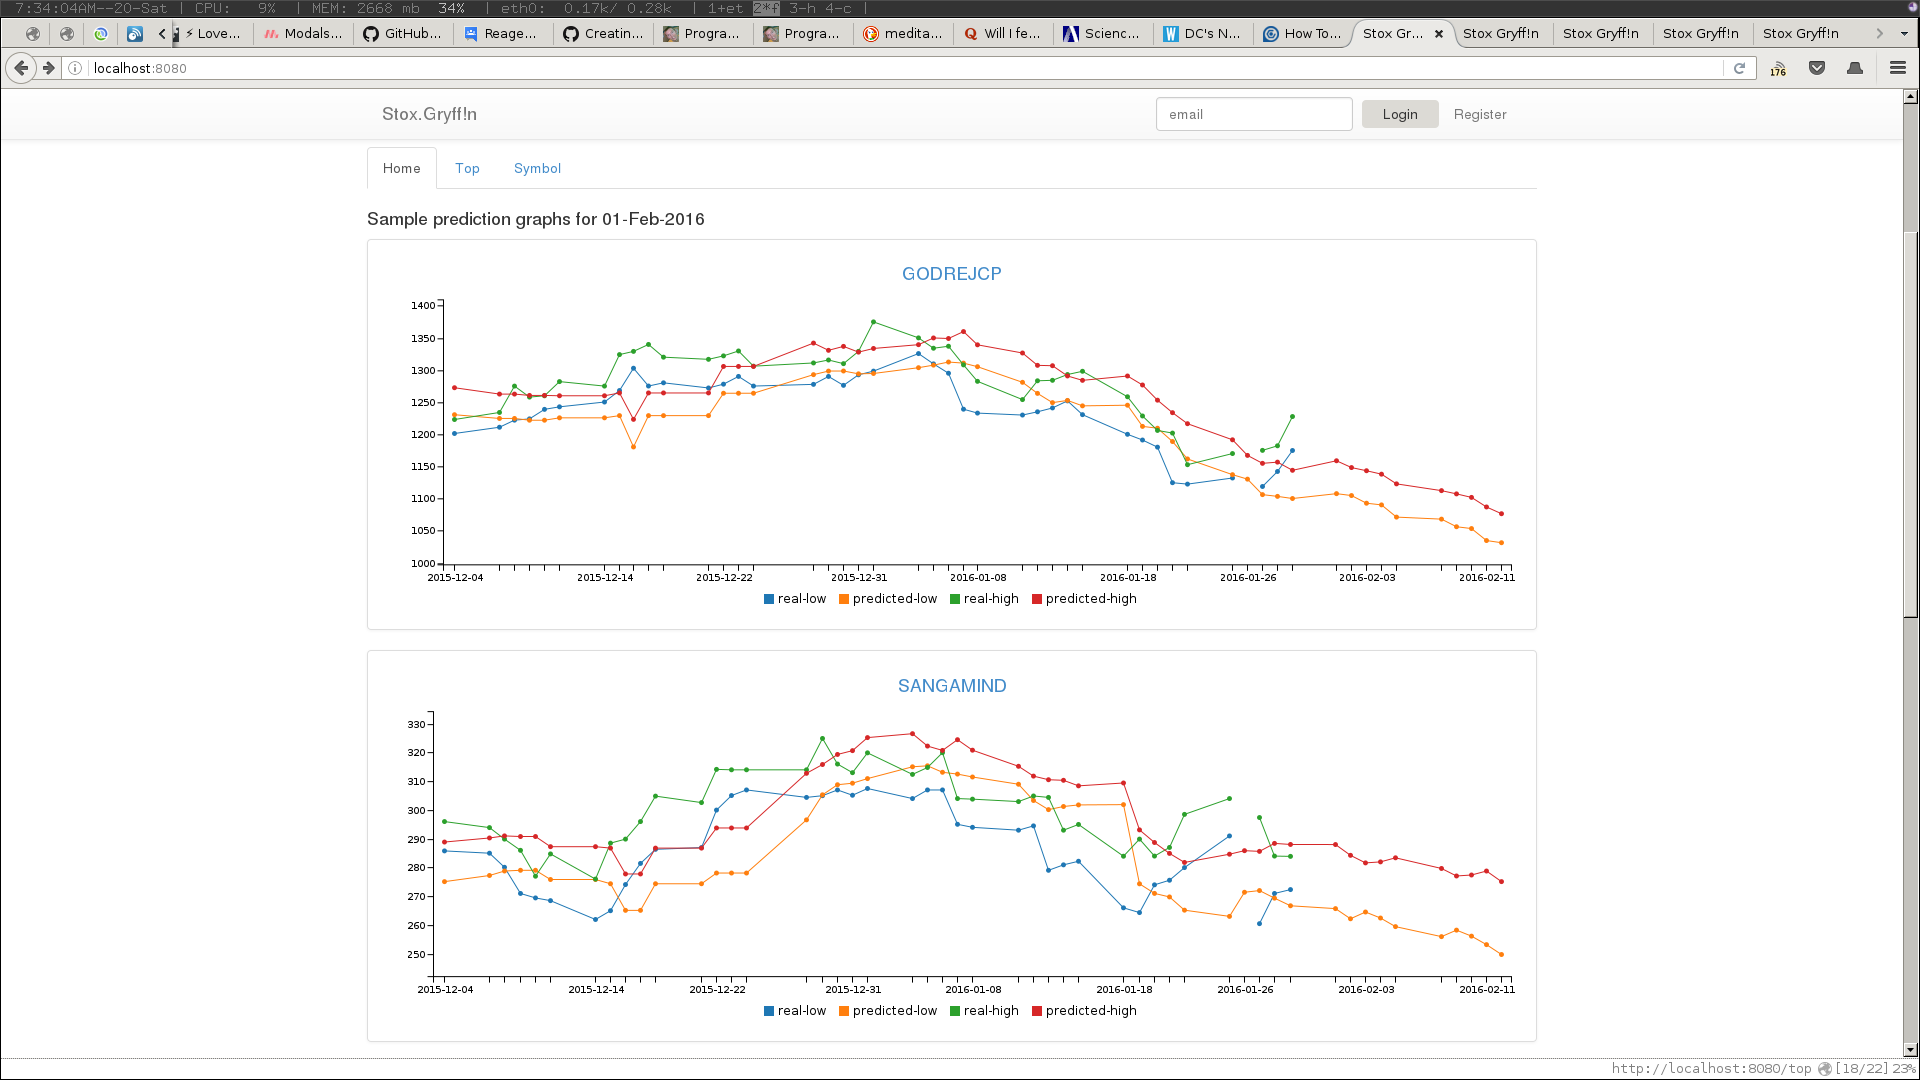
\includegraphics[height=5.4cm,width=10.8cm]{screenshot_2017-05-20_07-34-04.png}
\end{frame}
\begin{frame}
  \frametitle{Justdial}
  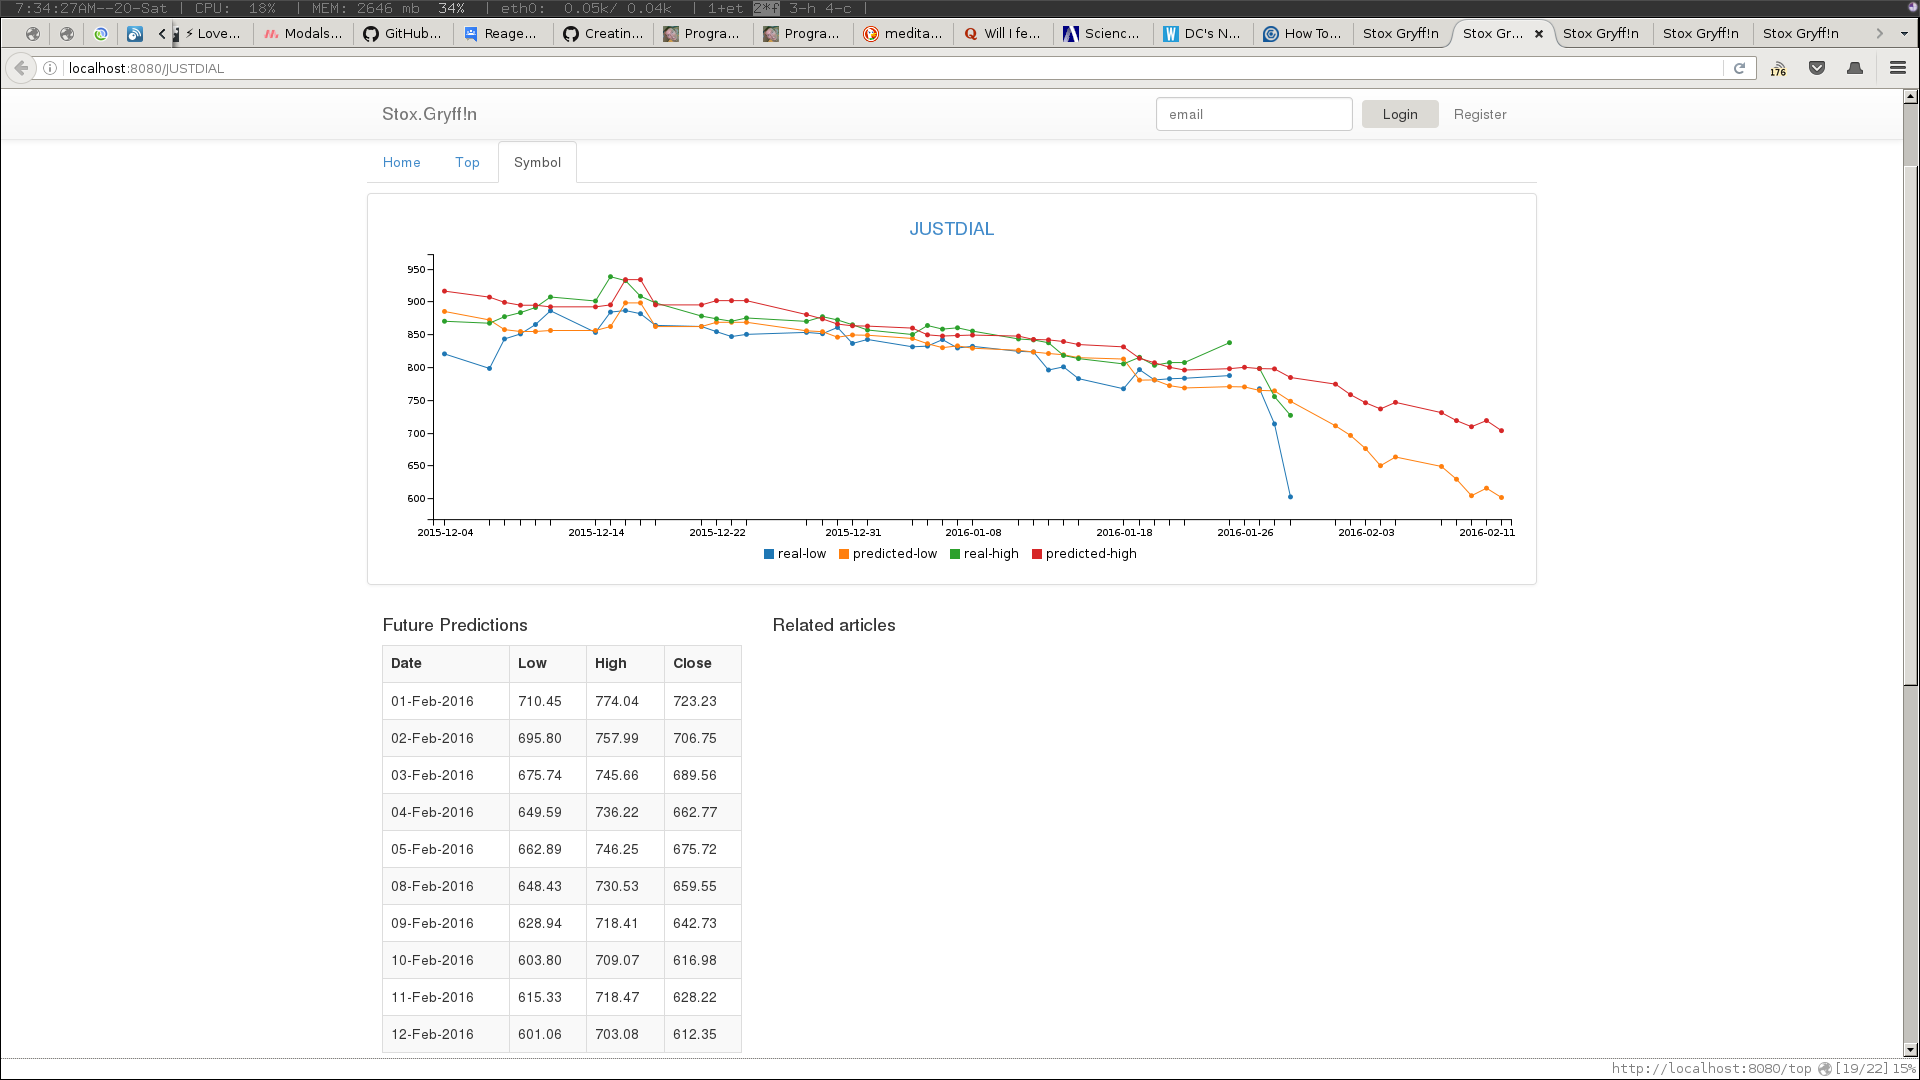
\includegraphics[height=5.4cm,width=10.8cm]{screenshot_2017-05-20_07-34-30.png}
\end{frame}
\begin{frame}
  \frametitle{GKWL Limited}
  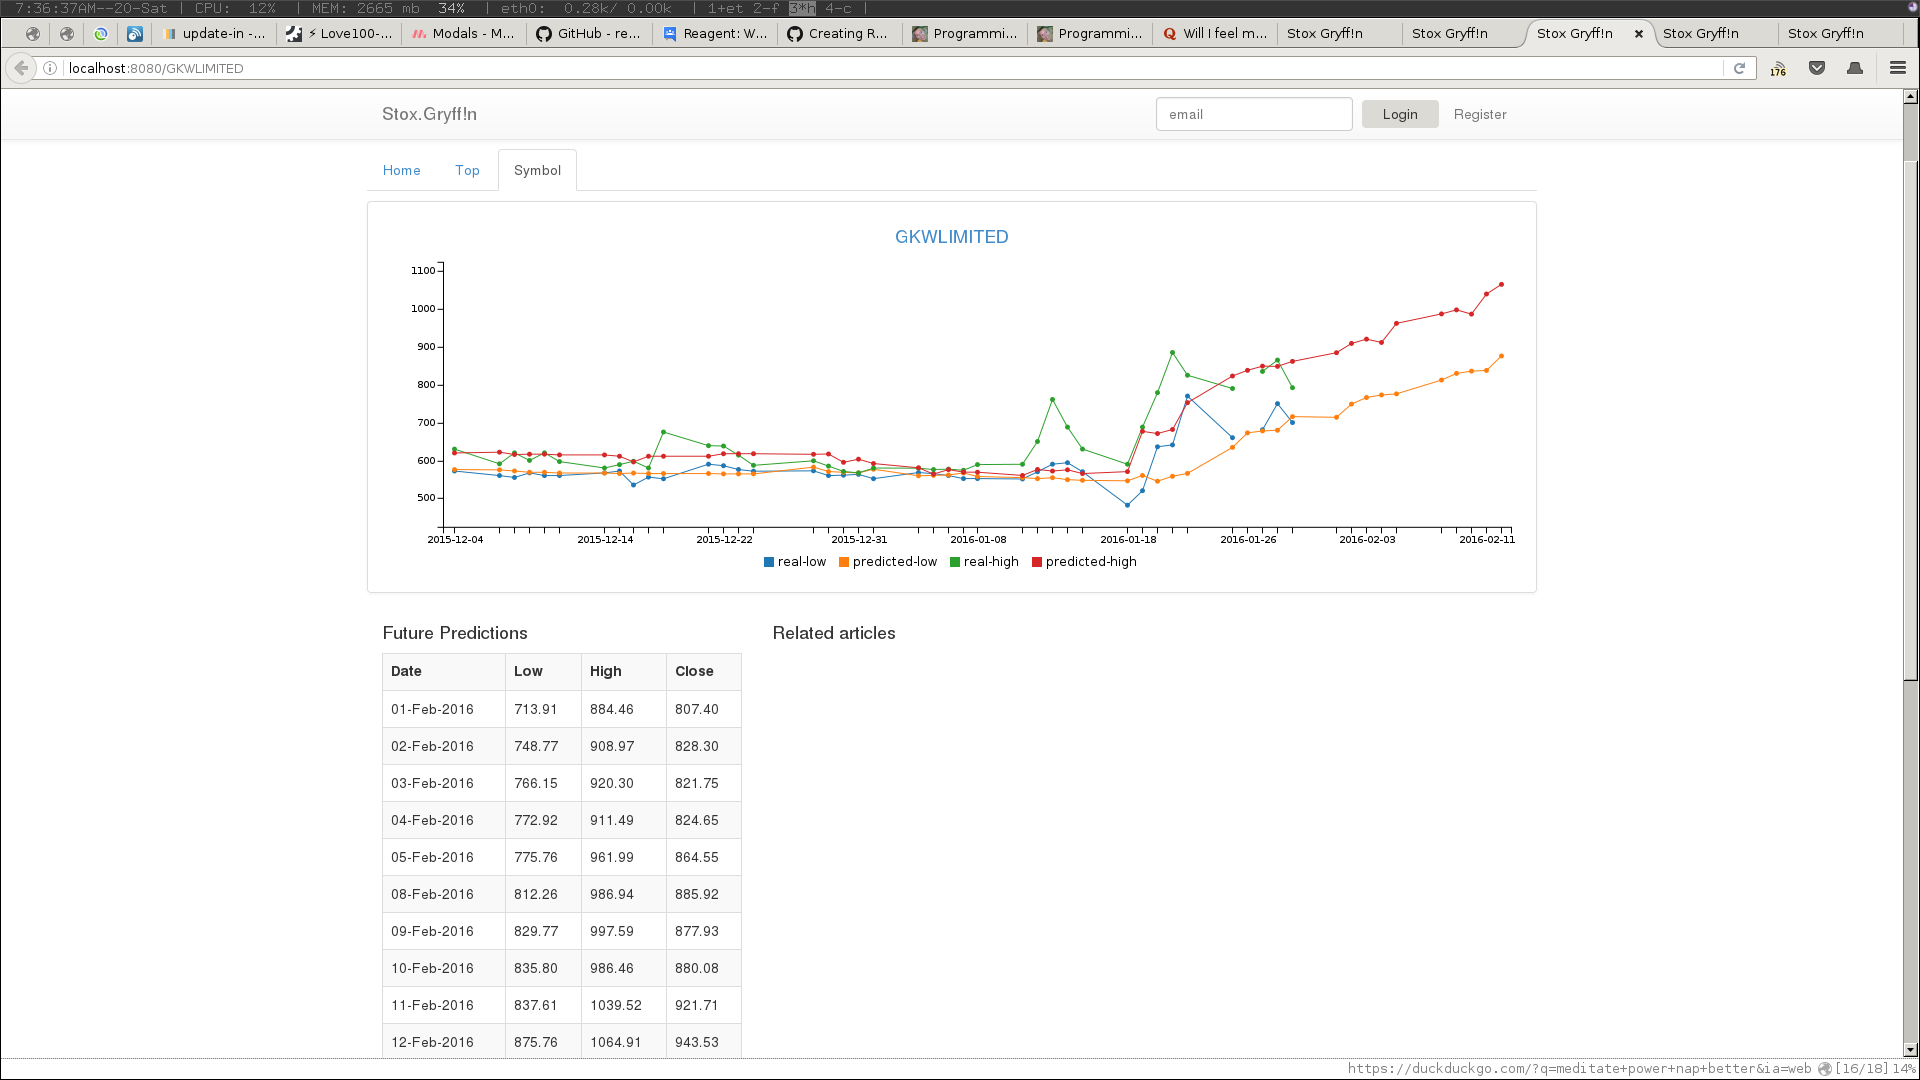
\includegraphics[height=5.4cm,width=10.8cm]{screenshot_2017-05-20_07-36-44.png}
\end{frame}
\begin{frame}
  \frametitle{Shrenuj}
  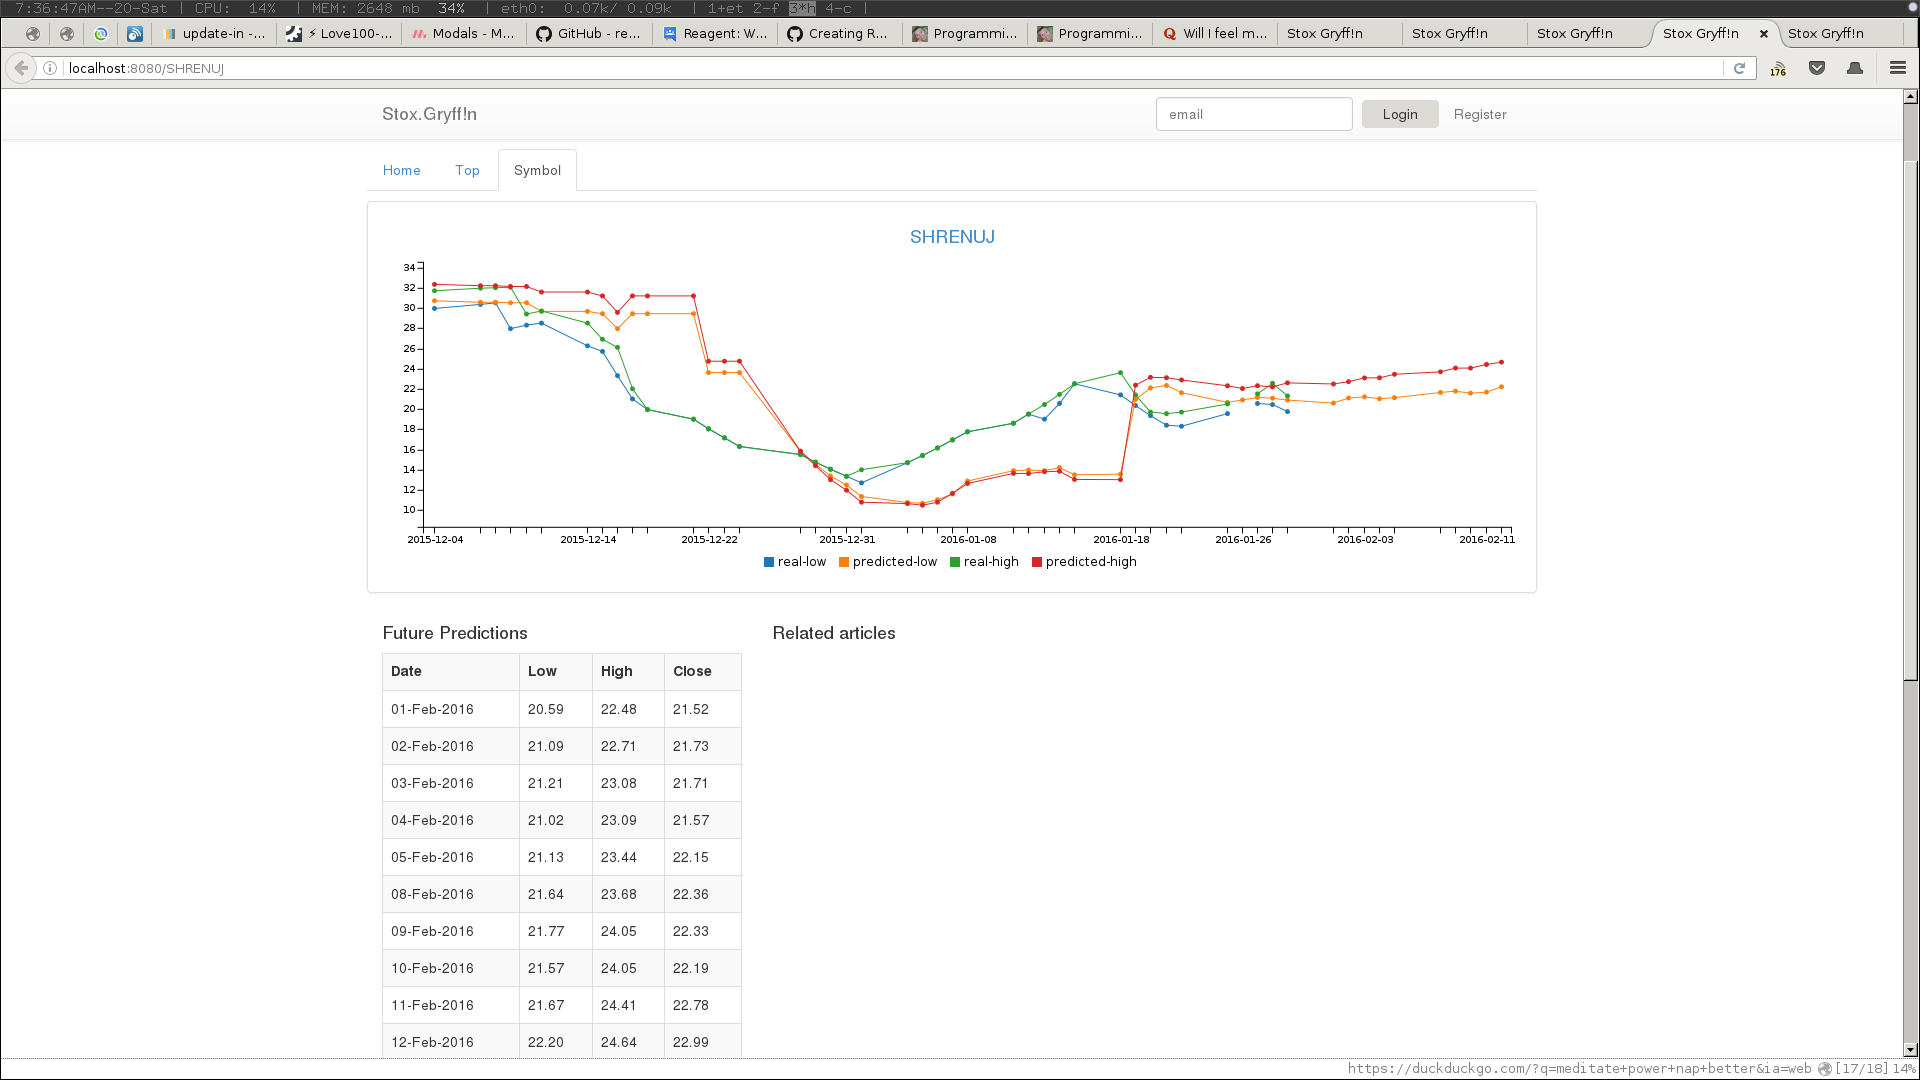
\includegraphics[height=5.4cm,width=10.8cm]{screenshot_2017-05-20_07-36-50.png}
\end{frame}
%% ----------
\subsection{Product : how}
\begin{frame}
  \frametitle{Server Architecture}
  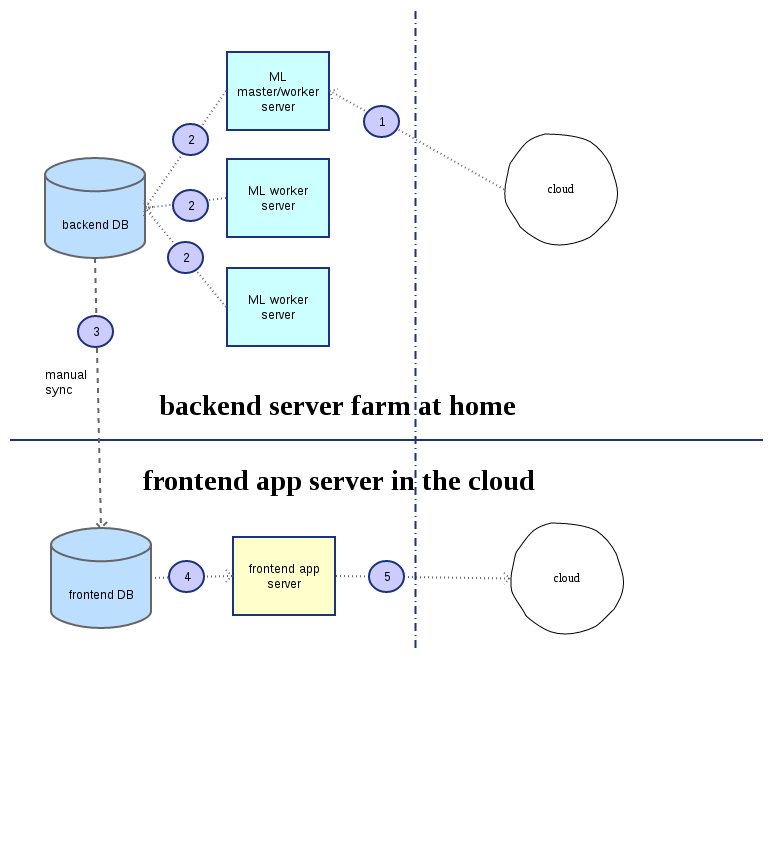
\includegraphics[height=7.4cm,width=10.8cm]{stox_architecture.png}
\end{frame}
\begin{frame}
  \frametitle{Data Flow Sequence}
  \begin{enumerate}
  \item \textit{ML master server}
    \begin{enumerate}
    \item fetch today's trading data from finance.yahoo.com
    \item normalize data and stores in DB
    \item trigger \textit{ML worker server}s to wake up and start processing data
    \end{enumerate}
  \item all \textit{ML worker server}s do predictions from models that were previously generated and stored
  \item once all processing is done, predicted data is moved from \textit{backend DB} to \textit{frontend DB}. this step is done \textit{manually} by me
  \item \textit{frontend app server} shows this data to clients
  \end{enumerate}
\end{frame}
\begin{frame}
  \frametitle{Technologies Used}
    \begin{itemize}
    \item clojure(script), Postgresql DB
    \item http://tinyurl.com/andrewngcoursera (Andrew Ng's coursera lectures on ML)
    \item ML libraries used
      \begin{itemize}
      \item Weka (http://www.cs.waikato.ac.nz/ml/weka/)
      \item Encog (http://www.heatonresearch.com/encog/)
      \end{itemize}
    \item currently popular ML libraries
      \begin{itemize}
      \item Caffe (http://caffe.berkeleyvision.org/)
      \item Keras (https://keras.io/ (high level UI over Theano, TensorFlow))
      \item Theano (http://www.deeplearning.net/software/theano/)
      \item TensorFlow (https://www.tensorflow.org/, created by Google)
      \item Torch (http://torch.ch/, used by Facebook)
      \end{itemize}
    \end{itemize}
\end{frame}
%% ----------
\subsection{Product : lessons}
\begin{frame}
  \frametitle{Machine Learning is hard to get right!}
  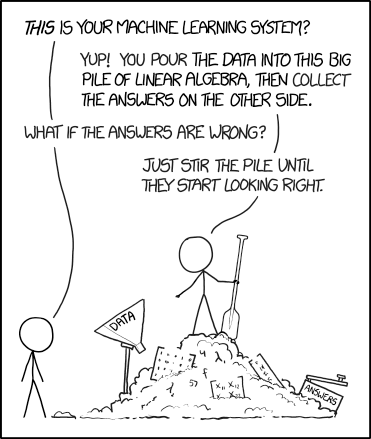
\includegraphics[height=5.4cm,width=5.4cm]{machine_learning.png}

https://xkcd.com/1838/
\end{frame}
\begin{frame}
  \frametitle{Lessons Learned}
  \begin{itemize}
  \item it is a great BTP or MTP or maybe even a PhD project
  \item extremely difficult to monetize unless you have a \textbf{team} of
    \begin{itemize}
    \item ML experts
    \item domain experts (for validating models)
    \item finance and marketing/sales (for monetization)
    \end{itemize}
  \item<2-> do \textbf{NOT} do it alone
  \end{itemize}
\end{frame}

%% -------------------------
%% Stuff I wish I knew at the begining of my career
\section{Stuff I wish I knew at the begining of my career}
\begin{frame}
  \begin{itemize}
  \item linux (mandatory for the software engineer)
  \item there is always something better out there
    \begin{itemize}
    \item c -$>$ java -$>$ python -$>$ php/js -$>$ common lisp -$>$ clojure
    \item notepad -$>$ vim -$>$ emacs
    \item manual testing -$>$ automated testing -$>$ continuous integration
    \end{itemize}
  \item don't underestimate yourself (you can do anything you wish to; take risks)
  \item don't try to do everything yourself (ask for help / collaborate)
  \item invest in your career
  \end{itemize}
\end{frame}
\begin{frame}
  read lots of books (fiction and non-fiction)

  some books that shaped me:
  \begin{itemize}
  \item Getting Things Done -- David Allen
  \item Mindset -- Carol Dweck
  \item Rich Dad Poor Dad -- Robert Kiyosaki
  \item Power of habits -- Charles Duhigg
  \item Peak -- Anders Ericsson
  \item Fountainhead -- Ayn Rand
  \item Hooked -- Nir Eyal (very highly recommended if you want to build products)
  \end{itemize}
\end{frame}
\begin{frame}
  \frametitle{The most important thing in this whole talk}
  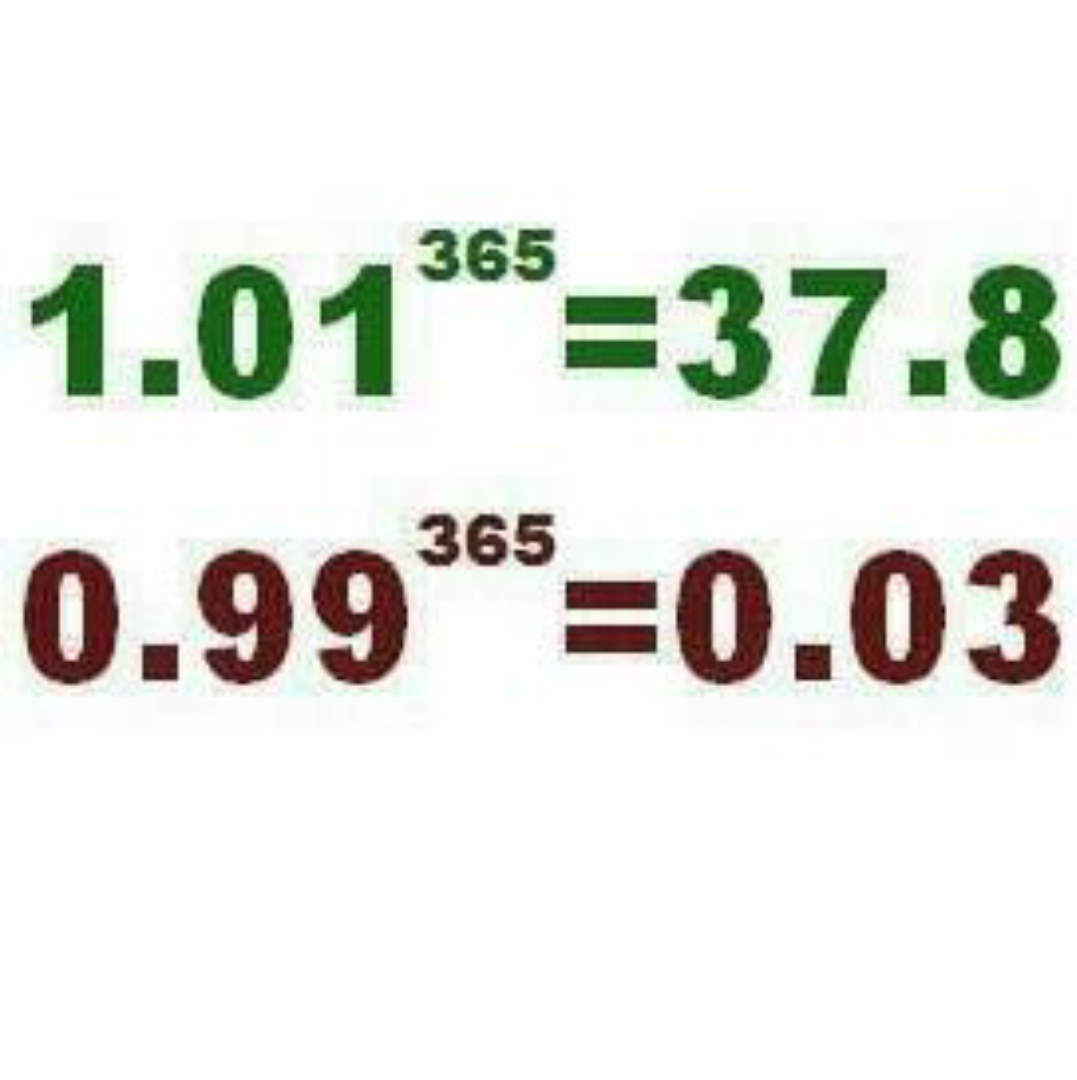
\includegraphics[height=5.4cm,width=10.8cm]{Screenshot_2017-05-20-09-10-52-736.png}

  http://jamesclear.com/the-1-percent-rule
\end{frame}

\end{document}
